\documentclass[10pt]{beamer}

\usetheme[progressbar=frametitle]{metropolis}
\usepackage{appendixnumberbeamer}
\usepackage[backend=biber,style=numeric,sorting=none]{biblatex}
\usepackage{booktabs}
\usepackage[scale=2]{ccicons}
\usepackage{siunitx}
\usepackage{pgfplots}
\usepgfplotslibrary{dateplot}
\usepackage{xspace}
\addbibresource{demo.bib}
\newcommand{\themename}{\textbf{\textsc{metropolis}}\xspace}

\title{Metropolis}
%\subtitle{A modern beamer theme}
% \date{\today}
\date{17 Luglio 2018}
\author{Davide Saccardo}
\institute{Università di Trento}
\titlegraphic{\hfill\includegraphics[height=1.5cm]{Sigillo_Università_di_Trento.pdf}}
%\includegraphics[height=1.5cm]{Sigillo_Università_di_Trento.pdf}

\begin{document}

\maketitle

\begin{frame}{Table of contents}
  \setbeamertemplate{section in toc}[sections numbered]
  \tableofcontents[hideallsubsections]
\end{frame}

\section{Introduzione}

\begin{frame}[fragile]{Obiettivi}
\begin{itemize}
	\item E' il Machine Learning applicabile per calcolare l'energia di ground state di un Condensato di Bose-Einstein (BEC)?
	\item Possiamo imparare qualcosa in più sulla Restricted Boltzmann Machine?
\end{itemize}

\end{frame}

\begin{frame}[fragile]{Ingredienti base}
	\begin{enumerate}
			\item Metodi Variational Monte Carlo per calcolare l'energia
			\item Funzione d'onda di prova rappresentata con Restricted Boltzmann Machine
			\item Parametri variazionali modificati con Stochastic Gradient Descent
	\end{enumerate}
\end{frame}

\begin{frame}[fragile]{Machine Learning}
	\begin{itemize}
		\item Set of algorithms to give computers the ability to learn to recognize images (e.g. plants, handwritten numbers) or data distribution
		\item Huge success in the last years: Google Translate, \dots
		\item Recent applications in physics with many-body problems such as Ising Model and Heisenberg model \footfullcite{carleoSolvingQuantumManybody2017}, with encouraging results
	\end{itemize}
\end{frame}

\begin{frame}[fragile]{Machine Learning}
	We represent our trial wave-function with a set of artificial Neural Networks. We call this way of representing the trail wave-function, Neural-Network Quantum State (NQS). The architecture selected is the Restricted Boltzmann Machine. The goal of the RBM is to learn the probability distribution of the simulated system. In quantum systems the probability distribution is the wave-function $\Psi$.
	
	\begin{figure}
		\centering
		\resizebox{10cm}{3.3333cm}{
			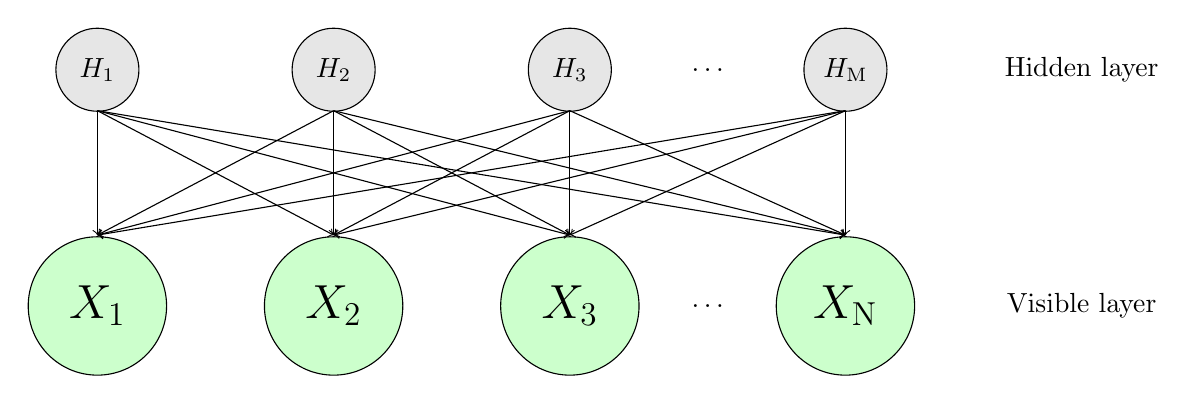
\begin{tikzpicture}
		\draw[black,fill=gray,fill opacity=0.2] (-4.5,0) circle (15pt) node[text=black, fill opacity=1] {$H_1$};
		\draw[black,fill=gray,fill opacity=0.2] (-1.5,0) circle (15pt) node[text=black, fill opacity=1] {$H_2$};
		\draw[black,fill=gray,fill opacity=0.2] (1.5,0) circle (15pt) node[text=black, fill opacity=1] {$H_3$};
		\node[draw, white, text=black] at (3.25,0) {$\dots$};
		\node[draw, white, text=black] at (8,0) {Hidden layer};
		\node[draw, white, text=black] at (8.0,-3) {Visible layer};
		\draw[black,fill=gray,fill opacity=0.2] (5,0) circle (15pt) node[text=black, fill opacity=1] {$H_\text{M}$};
		\draw[black,fill=green,fill opacity=0.2] (-4.5,-3) circle (25pt) node[text=black, fill opacity=1, align= center] {\LARGE $X_1$};
		\draw[black,fill=green,fill opacity=0.2] (-1.5,-3) circle (25pt) node[text=black, fill opacity=1] {\LARGE$X_2$};
		\draw[black,fill=green,fill opacity=0.2] (1.5,-3) circle (25pt) node[text=black, fill opacity=1] {\LARGE$X_3$};
		\node[draw, white, text=black] at (3.25,-3) {$\dots$};
		\draw[black,fill=green,fill opacity=0.2] (5,-3) circle (25pt) node[text=black, fill opacity=1] {\LARGE$X_\text{N}$};
		\draw[black,->] (-4.5,-0.52) to (-1.5,-2.1);
		\draw[black,->] (-4.5,-0.52) to (-4.5,-2.1);
		\draw[black,->] (-4.5,-0.52) to (1.5,-2.1);
		\draw[black,->] (-4.5,-0.52) to (5,-2.1);
		\draw[black,->] (-1.5,-0.52) to (-1.5,-2.1);
		\draw[black,->] (-1.5,-0.52) to (-4.5,-2.1);
		\draw[black,->] (-1.5,-0.52) to (1.5,-2.1);
		\draw[black,->] (-1.5,-0.52) to (5,-2.1);
		\draw[black,->] (1.5,-0.52) to (-1.5,-2.1);
		\draw[black,->] (1.5,-0.52) to (-4.5,-2.1);
		\draw[black,->] (1.5,-0.52) to (1.5,-2.1);
		\draw[black,->] (1.5,-0.52) to (5,-2.1);
		\draw[black,->] (5,-0.52) to (-1.5,-2.1);
		\draw[black,->] (5,-0.52) to (-4.5,-2.1);
		\draw[black,->] (5,-0.52) to (1.5,-2.1);
		\draw[black,->] (5,-0.52) to (5,-2.1);
		\end{tikzpicture}
	}
	\end{figure}
\end{frame}

\begin{frame}[fragile]{Machine Learning}
	
	The joint probability distribution of the RBM is defined as 
	\begin{equation*}
	F_{RBM}(\textbf{X},\textbf{H}) = \frac{1}{Z} \exp(-E(\textbf{X},\textbf{H})),
	\end{equation*}
	where \textbf{X} is the visible nodes and \textbf{H} is the hidden nodes. The quantity $Z$ represents the partition function or normalization constant of the system. 
	
	The quantity $E(\textbf{X},\textbf{H})$ is the function that specifies the relation between the visible and hidden nodes. It is called the energy of the node configuration. The choice of $E(\textbf{X},\textbf{H})$ is the heart of what sort of RBM we have.
	
\end{frame}

\begin{frame}[fragile]{Machine Learning}
	There are several types of RBM. Since, in our case, the visible nodes need to take continuous values, we choose the Gaussian-Binary RBM:
	\begin{equation*}
	E(\textbf{X},\textbf{H}) = \sum_i^{\text{N}}\frac{(X_i-a_i)^2}{2\sigma} - \sum_j^{\text{M}}b_jH_j + \sum_{ij}^{\text{N,M}}\frac{X_iw_{ij}H_j}{\sigma^2},
	\label{eq_rbm}
	\end{equation*} 
	To represent the wave-function, we use the so-called "marginal PDF" found by summing over all the hidden nodes:
	\begin{equation*}
	\Psi(\textbf{X}) = \sum_HF_{RBM}(\textbf{X},\textbf{H}) = \frac{1}{Z}\sum_H\exp(-E(\textbf{X},\textbf{H})).
	\end{equation*}
	Setting in the Gaussian-Binary RBM gives the final result
	\begin{equation*}
	\Psi(\mathbf{X}) = \frac{1}{Z} \exp\bigg[-\sum_i^{\text{N}} \frac{(X_i-a_i)^2}{2\sigma^2}\bigg]\prod_j^{\text{M}} \left(  1 + \exp\bigg[b_j +\sum_i^{\text{N}} \frac{X_iw_{ij}}{\sigma^2}\bigg]\right).
	\label{eq_psi}
	\end{equation*}
\end{frame}


\begin{frame}[fragile]{Condensato di Bose-Einstein}
\begin{itemize}
 	\item Stato della materia in cui gas diluiti di bosoni vengono sottoposti a una transizione di fase quando vengono raffreddati fino a basse temperature ($T\rightarrow 0\ \si{\kelvin}$). La maggior parte dei bosoni condensa nel ground state. Questo causa nuovi fenomeni quantistici come superfluidità e coerenza di fase.
 	\item Predetto da A. Einstein nel 1925 seguendo il lavoro del fisico indiano S. N. Bose (1924) sulla statistica dei bosoni. 
 	\item Verificati sperimentalmente nel 1995 dal team di Cornell e Wieman a Boulder con $^{87}$Rb e da Ketterle al MIT con $^{23}$Na raffreddati a temperature di $100\ \si{\nano\kelvin}$ attraverso laser cooling e evaporative cooling in trappole magneto-ottiche. Premio Nobel 2001.
\end{itemize}
\end{frame}
 

\begin{frame}[fragile]{Gross-Pitaevskii equation}
	Negli esperimenti sono stati utilizzati gas diluiti (e.g. atomi alcalini) e non uniformi perchè confinati in trappole magneto-ottiche. L'equazione di riferimento è l'equazione di Gross-Pitaevskii (GP): 
	\begin{equation*}
	\label{GP}
	i\hbar\frac{\partial \Psi (\mathbf{r},t)}{\partial t}=\bigg(-\frac{\hbar^2}{2m}\nabla^2+V(\mathbf{r})+g|\Psi(\mathbf{r},t)|^2\bigg)\Psi(\mathbf{r},t)
	\end{equation*}
	%\CIT %stringar
	dove $i=\sqrt{-1}, \hbar$ è la costante di Planck ridotta, $t$ è il tempi, $\Psi$ è la funzione d'onda del condensato, $\mathbf{r}$ rappresenta la posizione dei bosoni e $V$ è il potenziale esterno che intrappola i bosoni. La quantità $g$ è la costante di accoppiamento 
	\begin{equation*}
	g=\frac{4\pi\hbar^2a}{m}
	\end{equation*}
	dove $a$ is la lunghezza di scattering dell'onda s. Confronteremo le sue soluzioni in \cite{DalfString} con i nostri risultati. 
\end{frame}

\begin{frame}[fragile]{Motivazioni}
	La condizione di diluizione è data dal parametro $na^3$, dove $n$ è la densità del sistema.
	Quando il parametro è piccolo, GP funziona molto bene. Tuttavia ci sono esperimenti in cui il parametro supera tale valore. A qual punto è importante studiare il sistema con un approccio many-body. In letterature, troviamo molti papers in cui vengono utilizzati metodi Monte Carlo nel range diluito fino alla densità dell'$^4$He. Per esempio:
	\begin{enumerate}
		\item in \cite{vmcarticle}, Dubois e Glyde usano Variational Monte Carlo (VMC);
		\item in \cite{Giorgini}, Giorgini et al. usano Diffusion Monte Carlo (DMC);
		\item in \cite{Gruter}, Gr\"{u}ter et al. usano the path-integral Monte Carlo.
	\end{enumerate}  
	In this thesis, we use ML and we compare the results with GP equation since we consider a diluite system. Nevertheless, out of the diluite range, we note that ML results should be compared to the Monte Carlo ones which we have briefly mentioned above. 
\end{frame}


\section{Metodi}

\begin{frame}{Il sistema}
We consider a gas of $N_p$ bosons in spherical and elliptical harmonic oscillator potentials. The interaction between bosons in modeled by the hard-core model as in \cite{vmcarticle}. %We set $\hbar = m = 1$. 
The Hamiltonian of the system is 
\begin{equation}
H = \sum_{i=1}^{N_p}\left[ -\frac{1}{2}\frac{\hbar^2}{m}\nabla_i^2 + V_{ext}(\textbf{r}_i) \right]+ \sum_{i \neq k} V_{int}(r_{ik}),
\label{eq_hamilton}
\end{equation}
where $V_{ext}(\textbf{r})$ is the harmonic oscillator potential given by
\begin{equation*}
V_{ext}(\textbf{r})=\begin{cases}
\frac{1}{2}m\omega_{ho}^2r^2 &\text{Spherical}\\
\frac{1}{2}m\left[ \omega_{ho}^2 \left(x^2 + y^2 \right) + \omega_z^2 z^2\right] &\text{Elliptical}
\end{cases}
\end{equation*}
and $V_{int}(r_{ik})$ is the hard-shell interaction potential 
\begin{equation*}
V_{int}(r_{ik}) = \begin{cases}
0, & r_{ik} > a \\
\infty, & r_{ik} < a.
\end{cases}
\end{equation*}
The quantity $r_{ik} = |\textbf{r}_i-\textbf{r}_k|$ represents the distance between particle $i$ and $k$, while $a$ is the size of the interaction between particles. 
\end{frame}

\begin{frame}[fragile]{No interaction - spherical trap}
	When we set the interaction to be zero ($V_{int}=0$), we are left with a harmonic oscillator potential, where we consider a spherical shape for simplicity. In this case the solutions are known analytically. In general the energy is given by $E_n=\hbar\omega_{ho}(n+\frac{1}{2})$. The ground state is 
	\begin{equation*}
	E(N_p,D) = \frac{1}{2}\text{D} N_p\ \hbar\omega_{ho}.
	\label{analitica}
	\end{equation*}
	where D is the dimension of the system and $N_p$ is the number of particles. This case is useful to benchmark our code at the beginning.
\end{frame} 

\begin{frame}[fragile]{No interaction - elliptic trap}
	The interaction is still null ($V_{int}=0$), the trap now is considered to be elliptic.\\
	Let us introduce lengths in unit of $a_{ho}=\sqrt{\hbar/(m\omega_{ho)}}$, $r\rightarrow r/a_{ho}$ and energy in units of $\hbar\omega_{ho}$. The Hamiltonian can be rearranged as 
	\begin{equation*}
	\begin{split}
	H=\sum_{k=1}^{N_p}\frac{\hbar \omega_{ho}}{2}\bigg(-a_{ho}\nabla^2_{k}+a_{ho}{\hbar}\bigg[x^2_k+y^2_k+\frac{\omega^{2}_{z}}{\omega^{2}_{ho}}z^2_k\bigg]\bigg).
	\end{split}
	\end{equation*}
	We set $\lambda=\omega_z/\omega_{ho}$, we get
	\begin{equation}
	\label{ham}
	H=\sum_{k=1}^{N_p}\frac{1}{2}\bigg(-\nabla^2_{k}+V_{ext}(\mathbf{r}_k)\bigg)
	\end{equation}
	where $V_{ext}=x^2_k+y^2_k+\lambda^2 z^2_k$. As in \cite{DalfString}, we set $\lambda=\sqrt{8}$. In \cite{vmcarticle}, the energy of non-interacting bosons in this trap is shown to be
	\begin{equation*}
	\frac{E}{N}\rightarrow E_{ho}=\hbar\omega_{ho}\bigg(1+\frac{\lambda}{2}\bigg)=2.414\ \hbar\omega_{ho}.
	\end{equation*}
\end{frame}


\begin{frame}[fragile]{Interaction - elliptic trap}
At this point, we turn on the interaction $V_{int}\neq 0$ and we consider an elliptic trap. The Hamiltonian is

\begin{equation}
\label{ham2}
H=\sum_{k=1}^{N_p}\frac{1}{2}\bigg(-\nabla^2_{k}+V_{ext}(\mathbf{r}_k)\bigg)+\sum_{k<i}^{N_p} V_{int}(\mathbf{r}_k,\mathbf{r}_i).
\end{equation}
where $V_{ext}=x^2_k+y^2_k+\lambda^2 z^2_k$ and $\lambda=\sqrt{8}$ as above.	
\end{frame}




\metroset{titleformat frame=allsmallcaps}{
\begin{frame}{All small caps}
	This frame uses the \texttt{allsmallcaps} titleformat.

	\begin{alertblock}{Potential problems}
		As this titleformat also uses smallcaps you face the same problems as with the \texttt{smallcaps} titleformat. Additionally this format can cause some other problems. Please refer to the documentation if you consider using it.

		As a rule of thumb: Just use it for plaintext-only titles.
	\end{alertblock}
\end{frame}
}


\metroset{titleformat frame=allcaps}{
\begin{frame}{All caps}
	This frame uses the \texttt{allcaps} titleformat.

	\begin{alertblock}{Potential Problems}
		This titleformat is not as problematic as the \texttt{allsmallcaps} format, but basically suffers from the same deficiencies. So please have a look at the documentation if you want to use it.
	\end{alertblock}
\end{frame}
}

\section{Analisi dati}

\begin{frame}[fragile]{Typography}
      \begin{verbatim}The theme provides sensible defaults to
\emph{emphasize} text, \alert{accent} parts
or show \textbf{bold} results.\end{verbatim}

  \begin{center}becomes\end{center}

  The theme provides sensible defaults to \emph{emphasize} text,
  \alert{accent} parts or show \textbf{bold} results.
\end{frame}

\begin{frame}{Font feature test}
  \begin{itemize}
    \item Regular
    \item \textit{Italic}
    \item \textsc{SmallCaps}
    \item \textbf{Bold}
    \item \textbf{\textit{Bold Italic}}
    \item \textbf{\textsc{Bold SmallCaps}}
    \item \texttt{Monospace}
    \item \texttt{\textit{Monospace Italic}}
    \item \texttt{\textbf{Monospace Bold}}
    \item \texttt{\textbf{\textit{Monospace Bold Italic}}}
  \end{itemize}
\end{frame}

\begin{frame}{Lists}
  \begin{columns}[T,onlytextwidth]
    \column{0.33\textwidth}
      Items
      \begin{itemize}
        \item Milk \item Eggs \item Potatos
      \end{itemize}

    \column{0.33\textwidth}
      Enumerations
      \begin{enumerate}
        \item First, \item Second and \item Last.
      \end{enumerate}

    \column{0.33\textwidth}
      Descriptions
      \begin{description}
        \item[PowerPoint] Meeh. \item[Beamer] Yeeeha.
      \end{description}
  \end{columns}
\end{frame}
\begin{frame}{Animation}
  \begin{itemize}[<+- | alert@+>]
    \item \alert<4>{This is\only<4>{ really} important}
    \item Now this
    \item And now this
  \end{itemize}
\end{frame}
\begin{frame}{Figures}
  \begin{figure}
    \newcounter{density}
    \setcounter{density}{20}
    \begin{tikzpicture}
      \def\couleur{alerted text.fg}
      \path[coordinate] (0,0)  coordinate(A)
                  ++( 90:5cm) coordinate(B)
                  ++(0:5cm) coordinate(C)
                  ++(-90:5cm) coordinate(D);
      \draw[fill=\couleur!\thedensity] (A) -- (B) -- (C) --(D) -- cycle;
      \foreach \x in {1,...,40}{%
          \pgfmathsetcounter{density}{\thedensity+20}
          \setcounter{density}{\thedensity}
          \path[coordinate] coordinate(X) at (A){};
          \path[coordinate] (A) -- (B) coordinate[pos=.10](A)
                              -- (C) coordinate[pos=.10](B)
                              -- (D) coordinate[pos=.10](C)
                              -- (X) coordinate[pos=.10](D);
          \draw[fill=\couleur!\thedensity] (A)--(B)--(C)-- (D) -- cycle;
      }
    \end{tikzpicture}
    \caption{Rotated square from
    \href{http://www.texample.net/tikz/examples/rotated-polygons/}{texample.net}.}
  \end{figure}
\end{frame}
\begin{frame}{Tables}
  \begin{table}
    \caption{Largest cities in the world (source: Wikipedia)}
    \begin{tabular}{lr}
      \toprule
      City & Population\\
      \midrule
      Mexico City & 20,116,842\\
      Shanghai & 19,210,000\\
      Peking & 15,796,450\\
      Istanbul & 14,160,467\\
      \bottomrule
    \end{tabular}
  \end{table}
\end{frame}
\begin{frame}{Blocks}
  Three different block environments are pre-defined and may be styled with an
  optional background color.

  \begin{columns}[T,onlytextwidth]
    \column{0.5\textwidth}
      \begin{block}{Default}
        Block content.
      \end{block}

      \begin{alertblock}{Alert}
        Block content.
      \end{alertblock}

      \begin{exampleblock}{Example}
        Block content.
      \end{exampleblock}

    \column{0.5\textwidth}

      \metroset{block=fill}

      \begin{block}{Default}
        Block content.
      \end{block}

      \begin{alertblock}{Alert}
        Block content.
      \end{alertblock}

      \begin{exampleblock}{Example}
        Block content.
      \end{exampleblock}

  \end{columns}
\end{frame}
\begin{frame}{Math}
  \begin{equation*}
    e = \lim_{n\to \infty} \left(1 + \frac{1}{n}\right)^n
  \end{equation*}
\end{frame}
\begin{frame}{Line plots}
  \begin{figure}
    \begin{tikzpicture}
      \begin{axis}[
        mlineplot,
        width=0.9\textwidth,
        height=6cm,
      ]

        \addplot {sin(deg(x))};
        \addplot+[samples=100] {sin(deg(2*x))};

      \end{axis}
    \end{tikzpicture}
  \end{figure}
\end{frame}
\begin{frame}{Bar charts}
  \begin{figure}
    \begin{tikzpicture}
      \begin{axis}[
        mbarplot,
        xlabel={Foo},
        ylabel={Bar},
        width=0.9\textwidth,
        height=6cm,
      ]

      \addplot plot coordinates {(1, 20) (2, 25) (3, 22.4) (4, 12.4)};
      \addplot plot coordinates {(1, 18) (2, 24) (3, 23.5) (4, 13.2)};
      \addplot plot coordinates {(1, 10) (2, 19) (3, 25) (4, 15.2)};

      \legend{lorem, ipsum, dolor}

      \end{axis}
    \end{tikzpicture}
  \end{figure}
\end{frame}
\begin{frame}{Quotes}
  \begin{quote}
    Veni, Vidi, Vici
  \end{quote}
\end{frame}

{%
\setbeamertemplate{frame footer}{My custom footer}
\begin{frame}[fragile]{Frame footer}
    \themename defines a custom beamer template to add a text to the footer. It can be set via
    \begin{verbatim}\setbeamertemplate{frame footer}{My custom footer}\end{verbatim}
\end{frame}
}

\begin{frame}{References}
  Some references to showcase [allowframebreaks] \cite{knuth92,ConcreteMath,Simpson,Er01,greenwade93}
\end{frame}

\section{Conclusione}

\begin{frame}{Summary}

  Get the source of this theme and the demo presentation from

  \begin{center}\url{github.com/matze/mtheme}\end{center}

  The theme \emph{itself} is licensed under a
  \href{http://creativecommons.org/licenses/by-sa/4.0/}{Creative Commons
  Attribution-ShareAlike 4.0 International License}.

  \begin{center}\ccbysa\end{center}

\end{frame}

{\setbeamercolor{palette primary}{fg=black, bg=yellow}
\begin{frame}[standout]
  Questions?
\end{frame}
}

\appendix

\begin{frame}[fragile]{Backup slides}
  Sometimes, it is useful to add slides at the end of your presentation to
  refer to during audience questions.

  The best way to do this is to include the \verb|appendixnumberbeamer|
  package in your preamble and call \verb|\appendix| before your backup slides.

  \themename will automatically turn off slide numbering and progress bars for
  slides in the appendix.
\end{frame}

\begin{frame}[allowframebreaks]{References}
  %\bibliographystyle{abbrv}
  %\bibliography{demo}
  \printbibliography
\end{frame}

\end{document}
